%!TEX root=ast2016.tex

\begin{figure*}[t]
  \centering
  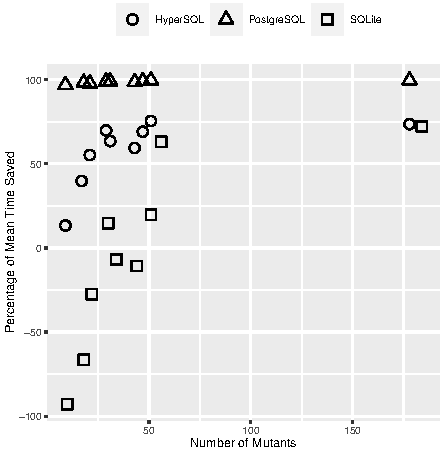
\includegraphics[scale=1.0]{graphics/graphic_scatterplot_nummutants_percentage.pdf}
  \caption{Scatter plot of the execution time for the original and virtual mutation analysis techniques.}
  \label{fig:graphic_bwplot_schema_analysistime_org_vm}

  {\small \justifying{ \noindent In this plot the box itself represents the interquartile range (IQR), or the measure of
      statistical dispersion that is the difference between the first and third quartiles. Furthermore, the upper
      whisker extends from the top of the box to the highest value that is within 1.5 times the IQR, the lower whisker
      goes from the bottom of the box to the lowest value within 1.5 times the IQR, and the thick horizontal line
      represents the median value. The boxes in this plot are noticeably compressed because there is little variance in
      the timings across the different configurations.  Since the results from running the original method on the
      \Postgres DBMS differ substantially from those with the other techniques and databases, all of the
      data values were log-transformed, thereby best revealing the relevant trends.} \par}

\end{figure*}
